\documentclass[a4paper]{scrartcl}
\usepackage[utf8]{inputenc}
\usepackage{fancyhdr}
\usepackage{enumitem}
\usepackage{tikz}
\usepackage{float}
\usepackage{multirow}
\usepackage{tabularx}

\title{Kompendium for Fellesprosjektet}

\subtitle{
TTM4100 - Kommunikasjon - Tjenester og nett \\
TDT4140 - Programvareutvikling \\
TDT4145 - Datamodellering og Databasesystemer \\
TDT4180 - Menneske-maskin-interaksjon
}

\lhead{Kompendium for Fellesprosjektet}
\rhead{TDT4140}

\author{
Redaktør Hans Moen \\
Revidert av Aleksander Vognild Burkow
}

\pagestyle{fancyplain}

\begin{document}

\maketitle
\thispagestyle{empty}
\newpage

\tableofcontents
\newpage

\section{Introduksjon til fellesprosjektet}
\subsection{Hva er ”fellesprosjektet”?}

Velkommen til fellesprosjektet for de fire fagene: TTM4100 - Kommunikasjon, TDT4140 - Systemutvikling, TDT4145 - Datamodellering og databasesystemer og TDT4180 - Menneske-maskin-interaksjon (MMI). Fellesprosjektet utgjør en del av det obligatoriske øvingsopplegget i disse fire fagene, og består av to store innleveringer i løpet av semesteret. Merk at studenter som kun tar noen av disse fire fagene, enten har en begrenset variant av fellesprosjektet, eller har egne obligatoriske øvinger innenfor hvert fag. Det er satt av i alt fire uker til fellesprosjektet – de to første ukene til planlegging og design, og de to neste ukene til implementering og testing. I disse to periodene vil det ikke være forelesninger i de fagene som er involvert i fellesprosjektet. 

Fellesprosjektet er viktig av flere grunner: Det gir muligheten til å lære og å praktisere teorien i fire fag, dere får erfaring med prosjektformen for organisering av arbeid, og dere får jobbe i grupper, med alt det måtte føre med seg av gleder og sorger. De fleste vil i ettertid huske fellesprosjektet som et strevsomt og givende fag, det har i hvert fall vært tilbakemeldingen fra tidligere studenter. 

Resten av dette kapittelet introduserer oppgaven og gir informasjon om relevante metoder og prosesser. Kapittel 2 forteller hva slags system vi skal utvikle og hva systemet skal brukes til. I kapittel 3 konkretiseres de funksjonelle kravene som stilles til systemet, dvs. alt som brukeren ønsker å kunne utføre. I kapittel 3 beskrives strukturen / arkitekturen til systemet, og andre krav som stilles til konstruksjonen, de ikke-funksjonelle kravene. I kapittel 4 detaljeres kravene som fellesprosjektet setter til sine innleveringer. I kapitel 5 detaljerer vi kraven som fellesprosjektet setter til MMI. Kapitel 6 lenker til viktige momenter for KTN delen av fellesprosjektet, som funksjonelle krav, krav til innleveringer i dette faget og en beskrivelse av planlagt løsning for kommunikasjonsdelen. Kapitel 7 beskriver databasedelen. 

I tillegg har kompendier et vedlegg som behandler UML (Vedlegg A). 

\subsection{Rammer for prosjektet}

Prosjektet tar sikte på å gi dere praktisk og realistisk erfaring i prosjektbasert systemutvikling, men rammen for faget tilsier at realismen blir begrenset1.
I arbeidslivet ville det innledningsvis i et prosjekt være ganske stor usikkerhet med tanke på hva som skal gjøres – for eksempel kundens behov og krav til systemet. Mye av utviklingsjobben vil være å analysere kundens problem, vurdere hvilken rolle og funksjoner et system bør ha for å bidra til å løse kundens problemer og om det hele tatt kunne løses på en effektiv måte, og så velge passende utviklingsmetoder, programmeringsspråk, verktøy og lignende. I fellesprosjektet er imidlertid frihetsgradene sterkt reduserende fordi:

\begin{enumerate}
\item
Med for stor frihet vil mange grupper kunne ta feil veivalg i starten, noe som gjør at de ikke greier å fullføre på en fornuftig måte. Selv blant profesjonelle programvareutviklere er en god del prosjekter langt fra vellykkede, og dere befinner dere ennå på et tidlig stadium i en lang utdanning.

\item
Hvis alle prosjekter får lov til å utvikle seg i helt ulike retninger, vil dette kreve veiledningskapasitet som vi verken har finanser eller personellressurser til. Det ville også være vanskelig å oppdrive reelle kunder for så mange grupper.

\end{enumerate}

Følgelig er det i dette prosjektet lagt klare begrensninger på hva og hvordan:

\begin{enumerate}
\item
Det finnes ingen ordentlig kunde. Kravene til produktet er spesifisert på forhånd. Det blir derfor ingen kravspesifikasjonsfase. Hovedvekten ligger på fasene konstruksjon, implementasjon og testing.

\item
Tidsfristene for levering av delprodukter er gitt av oss. Dermed påtvinges alle grupper en viss oppdeling av produktet og fast progresjon i arbeidet, noe som gjør det langt lettere for oss å hjelpe de av dere som får problem på et eller annet tidspunkt. Ulempe med dette er at utviklingsmodell kan fort tolkes som Fossefallsmodellinspirert mens de fleste (både studenter, aktører i næringslivet, og forskere) er enige i at Fossefallsmodellen er en utdatert modell. Det er viktig å understreke at faste tidsfrister og sekvensering av konstruksjon, implementasjon og testing er et pedagogisk valg.

\end{enumerate}

Prosjektet skal utføres i grupper à 4-6 personer. Gruppesammensetningen bestemmes av oss, uten hensyn til hvem dere helst ville ha ønsket å samarbeide med. Det gis ikke karakter, bare bestått/ikke-bestått (tilsvarende bokstavkarakterene A-E/F), og normalt evalueres hele gruppen under ett. I ekstreme tilfeller av ikke-deltagelse vil det bli aktuelt å stryke enkeltpersoner. Man må bestå fellesprosjektet for å få adgang til eksamen i de involverte fagene. Grupper eller personer som står i fare for å stryke, vil få advarsel to uker før siste innlevering – det skal ikke komme som et sjokk like før eksamen. Viss man gjør sitt beste, behøver man ikke være redd for at man ikke skal greie å bestå. Det lønner seg imidlertid å sikte mot bedre enn akkurat bestått karakter, siden den praktiske kunnskapen vil være nyttig i hvert fag sin eksamen, og i fag og oppgaver senere i studiet.
Vi bruker systemet (http://www.idi.ntnu.no/emner/fellesprosjekt/grupper/registrer.php3) for en effektiv deling i grupper. Ellers benytter Fellesprosjektet it’slearning for innleveringer.

\newpage

\subsection{Leveranser}

\begin{table}[h]
\begin{tabularx}{\textwidth}{ l X X l }

\hline
\hline
Fase & Innlevering & Beskrivelse & Frist \\
\hline

Fase 1
&
PU 1: Prosjektplan &
Prosjektplan i henhold til krav i kapitel 4.1 &
TBA \\

&
PU 2: Systemtestplan &
Systemtestplan i henhold til krav i kapitel 4.1 &
TBA \\

&
DB 1: Konseptuelt skjema &
ER-modell &
2014-03-06 \\

&
PU 3: Overordnet design &
Overordnet design &
TBA \\

&
MMI D2.1: Brukbarhetstesting &
Godkjenning av pilottest øving &
TBA \\

&
MMI D2.2 &
Rapport fra brukbarhetstest av papirprototyp &
TBA \\

Fase 2
&
KTN 1 &
Project plan (Se kap. 6.3.1). &
2014-03-03 \\

&
DB 2: Logisk databaseskjema &
SQL-script for oppretting av database &
2014-03-14 \\

&
PU 4: Programvare &
Implementasjon og testing av systemet &
TBA \\

&
MMI D3 &
Skjermdesign og konstruksjon. &
2014-03-14 \\

Fase 3
&
PU 5: Dokumentasjon &
Sluttrapport i henhold til krav i kapitel 4.3 &
TBA \\

&
KTN 2 &
Deliver a working implementation (Se kap. 6.3.2). &
2014-03-24 \\

\hline

\end{tabularx}
\caption{Deliverables for the Common project}
\end{table}

Den informasjonen dere finner i dette kompendiet var riktig i det kompendiet gikk i trykken. Det hender imidlertid at ting forandrer seg, inkludert innleveringsfristene, og derfor er det viktig at dere jevnlig sjekker for nye versjoner av kompendiet.

Lenker til respektive nettsted:
\begin{enumerate}
\item Fellesprosjektet: http://www.idi.ntnu.no/emner/fellesprosjekt

\item TTM4100 – Kommunikasjon, tjenester og nett: http://www.item.ntnu.no/fag/ttm4100/ 

\item TDT4140 - Programvareutvikling: http://www.idi.ntnu.no/emner/tdt4140/

\item TDT4145 - Datamodellering og databasesystemer: http://www.idi.ntnu.no/emner/tdt4145/

\item TDT4180 - MMI og grafikk: http://www.idi.ntnu.no/emner/tdt4180/
\end{enumerate}

\section{System for elektroniske kalendre}
\subsection{Oversikt over systemet}

Hver ansatt i Firma X skal ha en personlig kalender. Hver gruppe skal ha en gruppe kalender. En gruppe kan bestå av flere personer og også av subgrupper. En person kan være medlem av flere grupper. Alle kalenderne skal være lagret på en kalendertjener. De ansatte skal ha tilgang til kalenderne sine med en kalenderklient. Kalenderklienten kjører på en lokalmaskin som kommuniserer med kalendertjeneren over lokalnettet. Mange kalenderklienter kan være koblet opp mot kalendertjeneren samtidig. Sammen utgjør kalendertjeneren og kalenderklientene systemet som skal implementeres.
Figur \ref{fig:high-level-architecture}  viser et høynivå systemarkitektur over kalendersystemet.

\begin{figure}[H]
    \centering
    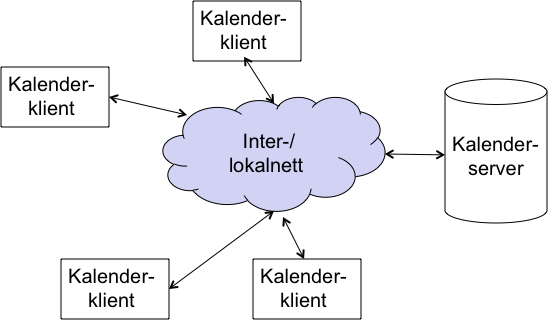
\includegraphics[scale=0.5]{resources/high-level-architecture.png}
    \caption{High level system architecture for calendar system}
    \label{fig:high-level-architecture}
\end{figure}

\subsection{Krav til kalendersystemet}

I tillegg til at de ansatte skal kunne planlegge dagene sine med å legge inn avtaler i kalenderne, er hensikten med kalendersystemet å forenkle innkalling til møter. I dag bruker de ansatte i Firma X mye tid på å koordinere intern-møter i organisasjonen. Tiden går med på å finne tidspunkt som passer for alle møtedeltakere, samt å reservere møterom. Kalendersystemet skal administrere innkalling til møter og reservasjon av møterom.

\begin{enumerate}

\item
Logge på. Ansatte får tilgang til kalendersystemet ved å logge seg på kalenderklienten med brukernavn og passord.

\item
Legge inn avtale. Ansatte skal kunne legge inn avtaler i kalenderene sine. En avtale legges inn på avtaledato med et start- og sluttidspunkt, samt en kort beskrivelse av avtalen ("Bil på verksted") og eventuelt sted for avtalen ("Strandveien Auto").

\item
Slette avtale. Ansatte skal kunne slette en avtale som ligger i en av kalenderene sine.

\item
Endre avtale. Ansatte skal kunne endre på en avtale som ligger i en av kalenderene sine. Alle feltene kan endres.

\item
Kalle inn til møte. En ansatt skal kunne kalle andre ansatte og grupper i Firma X inn til et møte. Den som kaller inn til møte kalles en møteleder. En ansatt skal kunne kalle inn til møte på samme måte som han/hun legger ny avtale inn i en kalender. I tillegg til feltene for en vanlig avtale, inneholder også møteinnkallingen en liste over innkalte møtedeltakere. 

\item
Motta møteinnkalling. Når en ansatt mottar innkalling til et møte, kan han/hun svare 'Godta' eller 'Forkast'. Ved å svare 'Godta', legges møteinnkallingen inn som en avtale i den innkalte ansattes kalender. Om den ansatte svarer 'Avslag', sendes svar tilbake til møtelederen om at innkallingen ikke er godtatt. Møteleder kan da velge å finne et nytt tidspunkt, avlyse møtet (se under) eller fjerne deltakeren fra innkallingslista.

\item
Endre møteinnkalling. Møteleder kan endre tidspunkt på en møteinnkalling. Det sendes da beskjed ut til alle møtedeltakerne, som kan svare 'Godta' eller 'Forkast'. Ved å svare 'Godta', endres avtalen i den innkalte ansattes kalender. Ved å svare 'Forkast' sendes beskjed ut til alle innkalte møtedeltakere. Møteleder kan da velge å finne et nytt tidspunkt eller å avlyse møtet (se under).

\item
Avlyse møte. Møteleder kan avlyse et møte. Det sendes da beskjed til alle møtedeltakerne, og systemet sletter møtet i deltakernes personlige kalender.

\item
Melde avbud for møte. En ansatt kan melde avbud på en møteinnkalling ved å slette avtalen i sin personlige kalender. Når en ansatt melder avbud, sendes melding til alle de andre møtedeltakerne. Møteleder kan da velge om møtet skal avlyses eller om han/hun skal endre tidspunkt på møtet.

\item
Reservere møterom. I stedet for å skrive inn sted for en avtale eller et møte, skal brukeren kunne reservere møterom. Kalendertjeneren skal lage en liste med tilgjengelige møterom (tilgjengelig betyr ikke reserverte) i tidsperioden for avtalen/møtet. Brukeren kan da velge møterom fra denne listen. Om en avtale med reservert møterom slettes, skal reservasjonen slettes på kalendertjeneren. Det samme gjelder for møter som avlyses.

\item
Visning. Kalenderklienten skal vise en ukekalender der alle avtaler og møter i den ansattes personlige kalender vises. Det skal være enkelt å bla mellom ukene.

\item
Spore møteinnkallinger. Kalenderklienten skal indikere i ukekalenderen om a) en møteinnkalling venter på svar fra en eller flere deltakere, b) en eller flere møtedeltakere har avslått møteinnkalling, eller c) om alle innkalte har godtatt møteinnkallingen.

\item
Vis flere kalendre. Det skal være mulig å vise andre ansattes avtaler sammen med sine egne i kalenderklienten.

\item
Alarm. Det skal være mulig for hver ansatt å konfigurere enhver avtale slik at avtalen genererer en alarm en gitt tid før møtet. 

\end{enumerate}

\subsection{Scenarioer}

Scenarioene er ikke en del av kravspesifikasjonen, men skisserer noen typiske bruksscenarier for kalendersystemet.

\begin{enumerate}

\item
En ansatt har invitert tre forretningsforbindelser til samtaler i Firma X sine lokaler. Den ansatte legger inn dette som en avtale i kalenderen sin, og får kalendersystemet til å booke et ledig møterom som er passe stort for fire deltakere.

\item
Jens kaller Beate, Morten og Finn til møte. Kalendersystemet  førstkommende fredag klokka 12 til 14. Kalendertjeneren sender melding til de tre Jens har kalt inn til møte. Morten er logget på systemet med en klient, og mottar øyeblikkelig melding om møteinnkallingen. Beate og Finn mottar meldingen neste gang de logger på.

\item
Beate avslår møteinnkallingen fordi hun har en annen avtale på det tidspunktet. Morten og Finn godtar innkallingen. Først forsøker Jens seg med å endre tidspunktet på møtet. Kalendertjeneren sender ny melding ut til møtedeltakerne. Denne gangen godtar både Beate og Finn møteinnkallingen, men Morten avslår. Jens velger å slette Morten fra møteinnkallingen. 

\item
Etter at Beate og Finn har godtatt møteinnkallingen blir Jens syk. Han sletter møtet fra kalenderen sin. Kalendertjeneren sender da melding til de to andre deltakerne om at møtet er avlyst. Beate og Finn mottar begge denne meldingen neste gang de logger seg på kalendersystemet.

\end{enumerate}

\newpage
\section{Arkitektur}
Dette kapitlet beskriver krav til konstruksjon eller systemdesign for fellesprosjektet. Konstruksjon av et system skal i prinsippet ikke påvirke de funksjonene som systemet har, men er relatert til de ikke-funksjonelle krav, for eksempel utvidbarhet, vedlikeholdbarhet, ytelse og skalerbarhet. Flerbrukerstøtte er et overordnet ikke-funksjonelt krav, dvs. at mange brukere skal kunne få tilgang til og endre de samme underliggende dataene, fra ulike maskiner på et nettverk.

Ved siden av de spesifiserte ikke-funksjonelle kravene, er det også en del generelle egenskaper ved konstruksjonen som er viktig, for eksempel at funksjoner har definerte grensesnitt i forhold til hverandre og at funksjoner en ønsker å endre på uavhengig av hverandre, ikke er for tett viklet sammen. Det er spesielt to typer koblinger vi er opptatt av å løse opp, nemlig koblinger mellom:

\begin{enumerate}

\item
Applikasjonsdata (modell) og grafisk brukergrensesnitt (GUI)

\item
Applikasjonsdata, slik de representeres mens applikasjonen er i bruk, og deres persistente representasjon på fil eller i en database. 

\end{enumerate}

Den andre av disse er konstruksjonsmessig knyttet til kravet om flerbrukerstøtte, som vi etter hvert skal se i de etterfølgende kapitlene. Kapittel 3.1 beskriver en overordnet systemarkitektur for de som har både SU, DB og KTN. For de som ikke tar DB, KTN og / eller MMI, vil det være noen endringer som er beskrevet i Kapittel 3.5.

\subsection{Trelags applikasjonsarkitektur}

Det er vanlig å dele applikasjoner i tre deler, med hver sin funksjon (se Figur 2):

\begin{enumerate}

\item
Brukergrensesnittet, i vårt tilfelle et GUI, er den delen som brukeren interagerer direkte med gjennom bl.a. skjerm, mus og tastatur. GUI gir brukeren mulighet for å navigere i og se på data og gir tilgang til funksjoner for å endre dataene. Strukturen på GUI er nært knyttet til strukturen til de dataene, slik den er beskrevet i f.eks. et UML klassediagram, men først og fremst basert på hva brukeren ønsker å gjøre. Implementasjonen av GUI gjøres ofte ved hjelp av et GUI-rammeverk og som regel i samme programmeringsspråk som applikasjonen forøvrig, i vårt tilfelle Java og Swing.

\item
Modellen er alle objektene i den kjørende applikasjonen som brukeren er interessert i å få tilgang til. Disse objektene eksisterer uavhengig av om GUI viser dem, og det er ikke umulig eller unaturlig å ha flere typer brukergrensesnitt som gir tilgang til de samme applikasjonsdataene, eller kun deler av disse. Modellen inneholder både data og regler for hvordan disse kan manipuleres, og sistnevnte kalles ofte applikasjonslogikk. Modellen vil typisk være beskrevet ved hjelp av UML klassediagram, som et ledd i analysearbeidet i forbindelse med. kravspesifikasjonen. Dersom en bruker et objektorientert språk som Java, vil både data og logikk implementeres vha. klasser. 

\item
Persistensdelen håndterer lagring av modellen mellom hver kjøring av applikasjonen, og er typisk støttet av en database eller et filsystem. Igjen er det ikke umulig eller unaturlig å tenke seg at de samme dataene kan lagres på ulike vis av en og samme applikasjon, f.eks. som en XML-fil, i en XML-database eller i en relasjonsdatabase. Førstnevnte passer bra for dokumentorienterte enbrukerapplikasjoner, sistnevnte passer bra for flerbrukerapplikasjoner med mer komplekse data og spørringer, og hvor det kan være behov for transaksjonshåndtering. Beskrivelsen av de persistente dataene er avhengig av den underliggende mekanismen, og kan være XML-dtd og –skjema og ER-diagram og SQL-skript.

\end{enumerate}

Ved konstruksjon er det viktig å tenke på både den interne strukturen i hver av de tre delene, som gjerne følger bestemte regler eller mønster for konstruksjon, og grensesnittet og samspillet mellom dem. Den interne strukturen i brukergrensesnittet og forholdet mellom brukergrensesnittet og modellen er en sentral del av MMI-faget. DB-faget tar for seg forholdet mellom applikasjonen og databasebasert persistens og struktur og egenskaper for databasen. Dersom disse tre delene av applikasjonen er skilt fra hverandre med et nettverk, har KTN-faget sitt å si om hvordan dette bør håndteres. SU-faget har den modellen/applikasjonslogikken og den overordnede strukturen eller arkitekturen, som sitt anliggende.

\subsection{Fra enbrukerapplikasjon til klient-tjener-arkitektur}

Applikasjonsarkitekturen som er beskrevet over, er et greit utgangspunkt for å konstruere en enbrukerapplikasjon. I dette prosjektet kan en forestille seg at en i første omgang støtter filbasert lagring med XML som format, som illustrert i Figur 3.

I en dokumentorientert applikasjon vil hele modellen bli lagret som en transaksjon, og grensesnittet mellom modellen, dvs. de to pilene, vil være nokså enkelt. Den venstre pilen representerer funksjonen modell-til-XML-oversetting, mens den høyre pilen tilsvarer den motsatte funksjonen XML-til-modell-oversetting. Merk at funksjonene håndterer kun hele modeller, så det er ikke behov for å oversette delmodeller i den ene eller andre retning. Det kan selvsagt være lurt å bryte funksjonene ned i mindre deler, basert på modellens struktur, men dette er konstruksjonsdetaljer som ikke påvirker grensesnittet representert ved pilene.

En ulempe med denne applikasjonsarkitekturen er at XML-filer ikke kan leses eller skrives over nettverket (med mindre en utnytter nettverkstøtten i filsystemet), f.eks. http- eller ftp-URL’er. Det skal imidlertid ikke så mye endring til for å håndtere dette, som vist i Figur 4.

Her vil klientapplikasjonen være så godt som uendret. Den eneste forskjellen er at lesing og skriving av XML-dokumentet skjer over nettverket, ved hjelp av en eller annen protokoll. Dersom en bruker URL-er til å adressere tjeneren og Java sin innebygde støtte for lesing og skriving til URL-oppkoblinger, så er det lite omkoding som trengs. I tillegg er det et stort poeng at endringen er intern i persistensdelen, så GUI og modellen er ikke berørt, kanskje bortsett fra dialogelementer for visning og innskriving av URL-en.
Tjeneren vil i dette tilfellet være nokså enkel, da den kun skal kunne ta i mot en oppkobling og kunne lese fra og skrive til nettverket og henholdsvis skrive til og lese fra fil.

Dersom en deler opp persistensdelen i en del som håndterer oversettingen til og fra XML og en del som håndterer lesing og skriving, er det relativt enkelt å få til en kombinasjon av disse to. Dette er vist i Figur 5.

Dette krever at overgangen mellom XML-oversettingen og lesing/skriving av XML-dokumentet er tydelig, f.eks. definert i et eget Java-grensesnitt og at en har klasser for filbasert og nettverksbasert I/O som implementerer dette grensesnittet. Dette tilsvarer forøvrig arkitekturen til først inkrement, med HTTP som nettverksprotokoll.

Selv om vi i de to siste figurene har innført en tjener, er tjeneren såpass enkel at arkitekturen ikke håndterer at flere brukere får tilgang til de samme dataene. Rollen til tjeneren er foreløpig kun knyttet til lagring og ikke til delt tilgang for flere klienter til felles data. For å få det til er det vesentlig at tjeneren også har et modell-lag og mekanismer for å håndtere delt tilgang. Figur 6 skisserer en arkitektur for å håndtere dette, men figuren forteller bare en del av historien.

Merk at modellene kan godt være implementert av akkurat de samme klassene og vi kan godt bruke XML som overføringsformat. I tillegg til å innføre et modell-lag i tjeneren, er det viktig å definere regler for samspillet mellom tjenerens modell og modellen i hver klient:

\begin{enumerate}

\item
Tjenerens modell er den offisielle modellen.

\item
Klientene må ved hver vesentlige endring lokalt, overføre endringen til tjeneren, for å unngå inkonsistens mellom lokal og offisiell modell.

\item
Tjeneren må, når den mottar endringer fra en klient, integrere endringene i sin modell, og videreformidle endringene til de andre klientene.

\item
Klientene må være beredt til å motta endringer fra tjeneren og integrere disse i sin egen lokale modell.

\end{enumerate}

Kommunikasjonen mellom tjeneren og klientene har altså som formål å sikre konsistens mellom lokale modeller og den tjenerens offisielle, og dataene som sendes over nettverket må være tilpasset dette formålet, for eksempel:

\begin{enumerate}

\item
Både tjeneren og klientene må kunne overføre fragmenter av modellen og ikke bare hele modellen som i enbrukerapplikasjonen

\item
Overføringen må inneholde informasjon om hva slags endring som skal gjøres i den andre enden, f.eks. slette, oppdatere eller opprette objekter

\item
En må kunne angi hvilke deler av den offisielle modellen som skal endres, f.eks. hvilket attributt som skal endre, hvilket objekt som skal slettes eller hvilken relasjon som skal opprettes

\end{enumerate}

Det som overføres i begge retninger mellom klient og tjener kan sees på som en kommando med tilhørende data, og en viktig del av designarbeidet er å definere kommandoene slik at dekker behovene over og bestemme hvordan de skal kodes i XML og formidles over HTTP.

Som vi ser er persistenslaget omdøpt til kommunikasjon i figuren over, men det betyr ikke at persistens er mindre viktig. Vi må fortsatt sikre at dataene overlever når applikasjonen avslutter, så persistensmekanismen må gjeninnføres, slik vi har vist i Figur 7.

For å sikre at modellen kan gjenopprettes hvis tjeneren krasjer, er det viktig at databasen blir oppdatert i takt med tjenerens modell. Hvilken som oppdateres først, modellen eller databasen, er en smakssak, men begge bør gjøres før klientene oppdateres, for å minimere muligheten for at krasj underveis. Det overordnede poenget er at det er databaseinnholdet som er grunnlaget for å gjenopprette modellen ved krasj eller vedlikehold av tjeneren. Derfor er databasen til syvende og sist mer ”offisiell” enn modellen i den kjørende tjeneren, siden det er den vi sitter igjen med når strømmen slås av.


\end{document}
